\documentclass{ML}
\usepackage{amsthm}
\usepackage{fontspec}
\usepackage[ruled,linesnumbered]{algorithm2e}
\usepackage{csvsimple}
\usepackage{booktabs}
\usepackage{longtable}

\setmonofont{Iosevka Nerd Font Mono}

\newtheorem{theorem}{定理}
% \newtheorem{proof}{证明}

% 姓名,学号
\infoauthor{冯云龙}{21B903004}

% 课程类型,实验名称
\infoexp{决策树ID3算法}

\begin{document}
\maketitle

\tableofcontents
\newpage

\section{实验介绍}

决策树(decision tree)是一种基本的分类与回归方法,此处主要讨论分类的决策树。

在分类问题中,表示基于特征对实例进行分类的过程,可以认为是if-then的集合,也可以认为是定义在特征空间与类空间上的条件概率分布。

\subsection{实验环境}

\begin{itemize}
	\item 操作系统:MacOS
	\item 编程语言:Python
	\item IDE:PyCharm
\end{itemize}

\section{决策树的特点}

\begin{itemize}
	\item 优点:计算复杂度不高,输出结果易于理解,对中间值的缺失不敏感,可以处理不相关特征数据。
	\item 缺点:可能会产生过度匹配的问题
	\item 适用数据类型:数值型和标称型

	\item 决策树学习的目标:根据给定的训练数据集构建一个决策树模型,使它能够对实例进行正确的分类。
	\item 决策树学习的本质:从训练集中归纳出一组分类规则,或者说是由训练数据集估计条件概率模型。
	\item 决策树学习的损失函数:正则化的极大似然函数
	\item 决策树学习的测试:最小化损失函数
	\item 决策树学习的目标:在损失函数的意义下,选择最优决策树的问题。
	\item 决策树原理和问答猜测结果游戏相似,根据一系列数据,然后给出游戏的答案。
\end{itemize}

\section{决策树的建立过程}
决策树通常有三个步骤:特征选择、决策树的生成、决策树的修剪。

用决策树分类:从根节点开始,对实例的某一特征进行测试,根据测试结果将实例分配到其子节点,此时每个子节点对应着该特征的一个取值,如此递归的对实例进行测试并分配,直到到达叶节点,最后将实例分到叶节点的类中。

\section{使用决策树做预测}

\begin{enumerate}
	\item 收集数据:可以使用任何方法。比如想构建一个相亲系统,我们可以从媒婆那里,或者通过参访相亲对象获取数据。根据他们考虑的因素和最终的选择结果,就可以得到一些供我们利用的数据了。
	\item 准备数据:收集完的数据,我们要进行整理,将这些所有收集的信息按照一定规则整理出来,并排版,方便我们进行后续处理。
	\item 分析数据:可以使用任何方法,决策树构造完成之后,我们可以检查决策树图形是否符合预期。
	\item 训练算法:这个过程也就是构造决策树,同样也可以说是决策树学习,就是构造一个决策树的数据结构。
	\item 测试算法:使用经验树计算错误率。当错误率达到了可接收范围,这个决策树就可以投放使用了。
	\item 使用算法:此步骤可以使用适用于任何监督学习算法,而使用决策树可以更好地理解数据的内在含义。
\end{enumerate}

\section{决策树的构造}
决策树学习的算法通常是一个递归地选择最优特征,并根据该特征对训练数据进行分割,使得各个子数据集有一个最好的分类的过程。这一过程对应着对特征空间的划分,也对应着决策树的构建。

\begin{enumerate}
	\item 开始:构建根节点,将所有训练数据都放在根节点,选择一个最优特征,按着这一特征将训练数据集分割成子集,使得各个子集有一个在当前条件下最好的分类。
	\item 如果这些子集已经能够被基本正确分类,那么构建叶节点,并将这些子集分到所对应的叶节点去。
	\item 如果还有子集不能够被正确的分类,那么就对这些子集选择新的最优特征,继续对其进行分割,构建相应的节点,如果递归进行,直至所有训练数据子集被基本正确的分类,或者没有合适的特征为止。
	\item 每个子集都被分到叶节点上,即都有了明确的类,这样就生成了一颗决策树。
\end{enumerate}

\section{决策树算法}

\subsection{ID3}

ID3算法中采取信息增益这个量来作为纯度的度量,每次选取信息增益最大的特征进行分裂。

信息熵是度量样本集合不确定度(纯度)的最常用的指标,它是代表随机变量的复杂度,条件熵代表在某一个条件下,随机变量的复杂度。而信息增益恰好是:信息熵-条件熵。

我们看如下定义:

\begin{itemize}
	\item 当前样本集合 $D$ 中第 $k$ 类样本所占的比例为 $p_k$ ,则 D 的信息熵定义为:$$ Ent(D) = - \sum_{k \in K} p_k \log_2(p_k) $$
	\item 离散属性 $a$ 有 $v$ 个可能的取值 ${a_1,a_2,\dots,a_V}$;样本集合中,属性 $a$ 上取值为 $a_v$ 的样本集合,记为 $D_v$。
	\item 用属性 $a$ 对样本集 $D$ 进行划分所获得的“信息增益”:$$Gain(D,a) = Ent(D) - \sum_{v \in V} \frac{ |D^v| }{ |D| Ent(D^v) }$$
	\item 信息增益表示得知属性 a 的信息而使得样本集合不确定度减少的程度
\end{itemize}

\begin{longtable}[c]{@{}cccccccc@{}}
	\toprule
	编号 & 色泽 & 根蒂 & 敲声 & 纹理 & 脐部 & 触感 & 好瓜 \\* \midrule
	\endfirsthead
	%
	\multicolumn{7}{c}%
	{{\bfseries 接表 \thetable}}                          \\
	\toprule
	色泽 & 根蒂 & 敲声 & 纹理 & 脐部 & 触感 & 好瓜        \\* \midrule
	\endhead
	%
	\bottomrule
	\endfoot
	%
	\endlastfoot
	%
	1    & 青绿 & 蜷缩 & 浊响 & 清晰 & 凹陷 & 硬滑 & 是   \\
	2    & 乌黑 & 蜷缩 & 沉闷 & 清晰 & 凹陷 & 硬滑 & 是   \\
	3    & 乌黑 & 蜷缩 & 浊响 & 清晰 & 凹陷 & 硬滑 & 是   \\
	4    & 青绿 & 蜷缩 & 沉闷 & 清晰 & 凹陷 & 硬滑 & 是   \\
	5    & 浅白 & 蜷缩 & 浊响 & 清晰 & 凹陷 & 硬滑 & 是   \\
	6    & 青绿 & 稍蜷 & 浊响 & 清晰 & 稍凹 & 软粘 & 是   \\
	7    & 乌黑 & 稍蜷 & 浊响 & 稍糊 & 稍凹 & 软粘 & 是   \\
	8    & 乌黑 & 稍蜷 & 浊响 & 清晰 & 稍凹 & 硬滑 & 是   \\
	9    & 乌黑 & 稍蜷 & 沉闷 & 稍糊 & 稍凹 & 硬滑 & 否   \\
	10   & 青绿 & 硬挺 & 清脆 & 清晰 & 平坦 & 软粘 & 否   \\
	11   & 浅白 & 硬挺 & 清脆 & 模糊 & 平坦 & 硬滑 & 否   \\
	12   & 浅白 & 蜷缩 & 浊响 & 模糊 & 平坦 & 软粘 & 否   \\
	13   & 青绿 & 稍蜷 & 浊响 & 稍糊 & 凹陷 & 硬滑 & 否   \\
	14   & 浅白 & 稍蜷 & 沉闷 & 稍糊 & 凹陷 & 硬滑 & 否   \\
	15   & 乌黑 & 稍蜷 & 浊响 & 清晰 & 稍凹 & 软粘 & 否   \\
	16   & 浅白 & 蜷缩 & 浊响 & 模糊 & 平坦 & 硬滑 & 否   \\
	17   & 青绿 & 蜷缩 & 沉闷 & 稍糊 & 稍凹 & 硬滑 & 否   \\* \bottomrule
	\caption{西瓜数据集}\label
	{tab:my-table}                                        \\
\end{longtable}

查看上面的例子,正例占$\frac{8}{17}$,反例占$\frac{9}{17}$,根节点的信息熵为$$Ent(D)=-(\frac{8}{17}\log_2{\frac{8}{17}} + {\frac{9}{17}}\log_2{\frac{9}{17}})=0.998$$

计算当前属性集合\{色泽,根蒂,敲声,纹理,脐部,触感\}中每个属性的信息增益,例如色泽有3个可能的取值:
\begin{itemize}
	\item D1(色泽=青绿) = \{1, 4, 6, 10, 13, 17\},正例 $\frac{3}{6}$,反例 $\frac{3}{6}$,信息熵$Ent(D^1)=1.000$

	\item D2(色泽=乌黑) = \{2, 3, 7, 8, 9, 15\},正例 $\frac{4}{6}$,反例 $\frac{2}{6}$,信息熵$Ent(D^1)=0.918$

	\item D3(色泽=浅白) = \{5, 11, 12, 14, 16\},正例 $\frac{1}{5}$,反例 $\frac{4}{5}$,信息熵$Ent(D^1)=0.722$
\end{itemize}

那么我们可以得到
\begin{align*}
	Gain(D,\text{色泽}) & = Ent(D) - \sum_{v \in V} \frac{ |D^v| }{ |D| Ent(D^v) }                \\
	                    & = 0.998 - (\frac{6}{17}*1.000 + \frac{6}{17}*0.918 +\frac{5}{17}*0.722) \\
	                    & = 0.109
\end{align*}

同理可得
\begin{align*}
	Gain(D, \text{色泽}) & = 0.108 &
	Gain(D, \text{根蒂}) & = 0.143   \\
	Gain(D, \text{敲声}) & = 0.141 &
	Gain(D, \text{纹理}) & = 0.381   \\
	Gain(D, \text{脐部}) & = 0.289 &
	Gain(D, \text{触感}) & = 0.006
\end{align*}

于是我们找到了信息增益最大的属性纹理,它的$Gain(D, \text{纹理}) = 0.38$最大。
于是我们选择的划分属性为“纹理”,如下所示:

\begin{figure}[htbp]
	\centering
	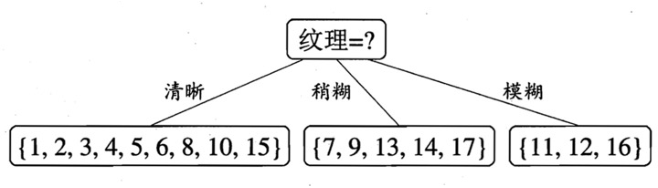
\includegraphics[width=0.7\textwidth]{media/DecisionTree/gain_start}
\end{figure}

于是,我们可以得到了三个子结点,对于这三个子节点,我们可以递归的使用刚刚找信息增益最大的方法进行选择特征属性,最终建立一棵决策树:

\begin{figure}[H]
	\centering
	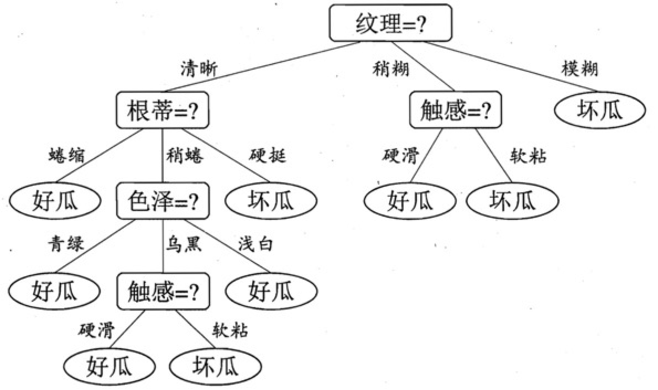
\includegraphics[width=0.7\textwidth]{media/DecisionTree/gain_final}
\end{figure}

在ID3决策树算法中,我们使用信息增益作为标准来选择特征:即如果选择一个特征后,信息增益最大(信息不确定性减少的程度最大),那么我们就选取这个特征。

\subsection{C4.5}

我们从上面求解信息增益的公式中,其实可以看出,信息增益准则其实是对可取值数目较多的属性有所偏好!

现在假如我们把数据集中的“编号”也作为一个候选划分属性。我们可以算出“编号”的信息增益是0.998。

因为每一个样本的编号都是不同的(由于编号独特唯一,条件熵为0了,每一个结点中只有一类,纯度非常高啊),也就是说,来了一个预测样本,你只要告诉我编号,其它特征就没有用了,这样生成的决策树显然不具有泛化能力。

C4.5算法就对这个问题进行了改进,它每次进行选取特征属性的时候,不再使用ID3算法的信息增益,而是使用信息增益率作为选择的标准。

首先我们来看信息增益率的公式:

$$IV = - \sum^V_{v=1} \frac{ |D^v| }{ |D| } log2( \frac{ |D^v| }{ |D| })$$
$$GainRatio(D,a) = \frac{ Gain(D,a) }{ IV }$$

信息增益率=信息增益/IV(a),说明信息增益率是信息增益除了一个属性a的固有值得来的。

我们一开始分析到,信息增益准则其实是对可取值数目较多的属性有所偏好!(比如上面提到的编号,可能取值是实例个数,最多了,分的类别越多,分到每一个子结点,子结点的纯度也就越可能大,因为数量少了嘛,可能在一个类的可能性就最大)。

但是刚刚我们分析到了,信息增益并不是一个很好的特征选择度量。于是我们引出了信息增益率。有了IV(a)这个分母之后,我们可以看到增益率准则其实对可取类别数目较少的特征有所偏好!毕竟分母越小,整体越大。

C4.5算法不直接选择增益率最大的候选划分属性,候选划分属性中找出信息增益高于平均水平的属性(这样保证了大部分好的的特征),再从中选择增益率最高的(又保证了不会出现编号特征这种极端的情况)。

\appendix

\section{源代码}

\inputminted[breaklines=true,frame=lines,mathescape=true]{python}{../decision_tree.py}

\end{document}
